%!TEX root = ../../../report.tex
\section{PCBs and wiring} % (fold)
\label{sec:pcbs_and_wiring}
In order to reduce weight and inertias in the section \ref{ssub:extension_pcbs} presents an extension board that interfaces between the motor and the BLDC electronics.
With a 1.8 meter long wiring used to extend the connection, the purpose of the extension PCBs are to be mounted over the joints, close enough to the motors so that their original wiring can be used, as in Figure \ref{fig:pcb2}, and transfer the signals to the motor board out of the structure, as in Figure \ref{fig:electronics1}.

New Molex connectors have been soldered to the original boards in order to implement these extensions, as shown in Figure \ref{fig:electronics2} within the final arrangement of the motor boards and the main processor board.
A distinctive color has been chosen for the wiring of each motor just to ease the task of arranging the final configuration.
Every motor board is labeled with the name of the joint it drives and matched to the appropriate address from the main processor by software, as explained in \ref{sub:ros_control_hardware_locokit_interface}.
This means that if a BLDC motor board is going to be changed, both its physical connection, label and internal address have to be changed accordingly.


\begin{figure}[ht]
\centering
  \begin{subfigure}[b]{0.4\textwidth}
    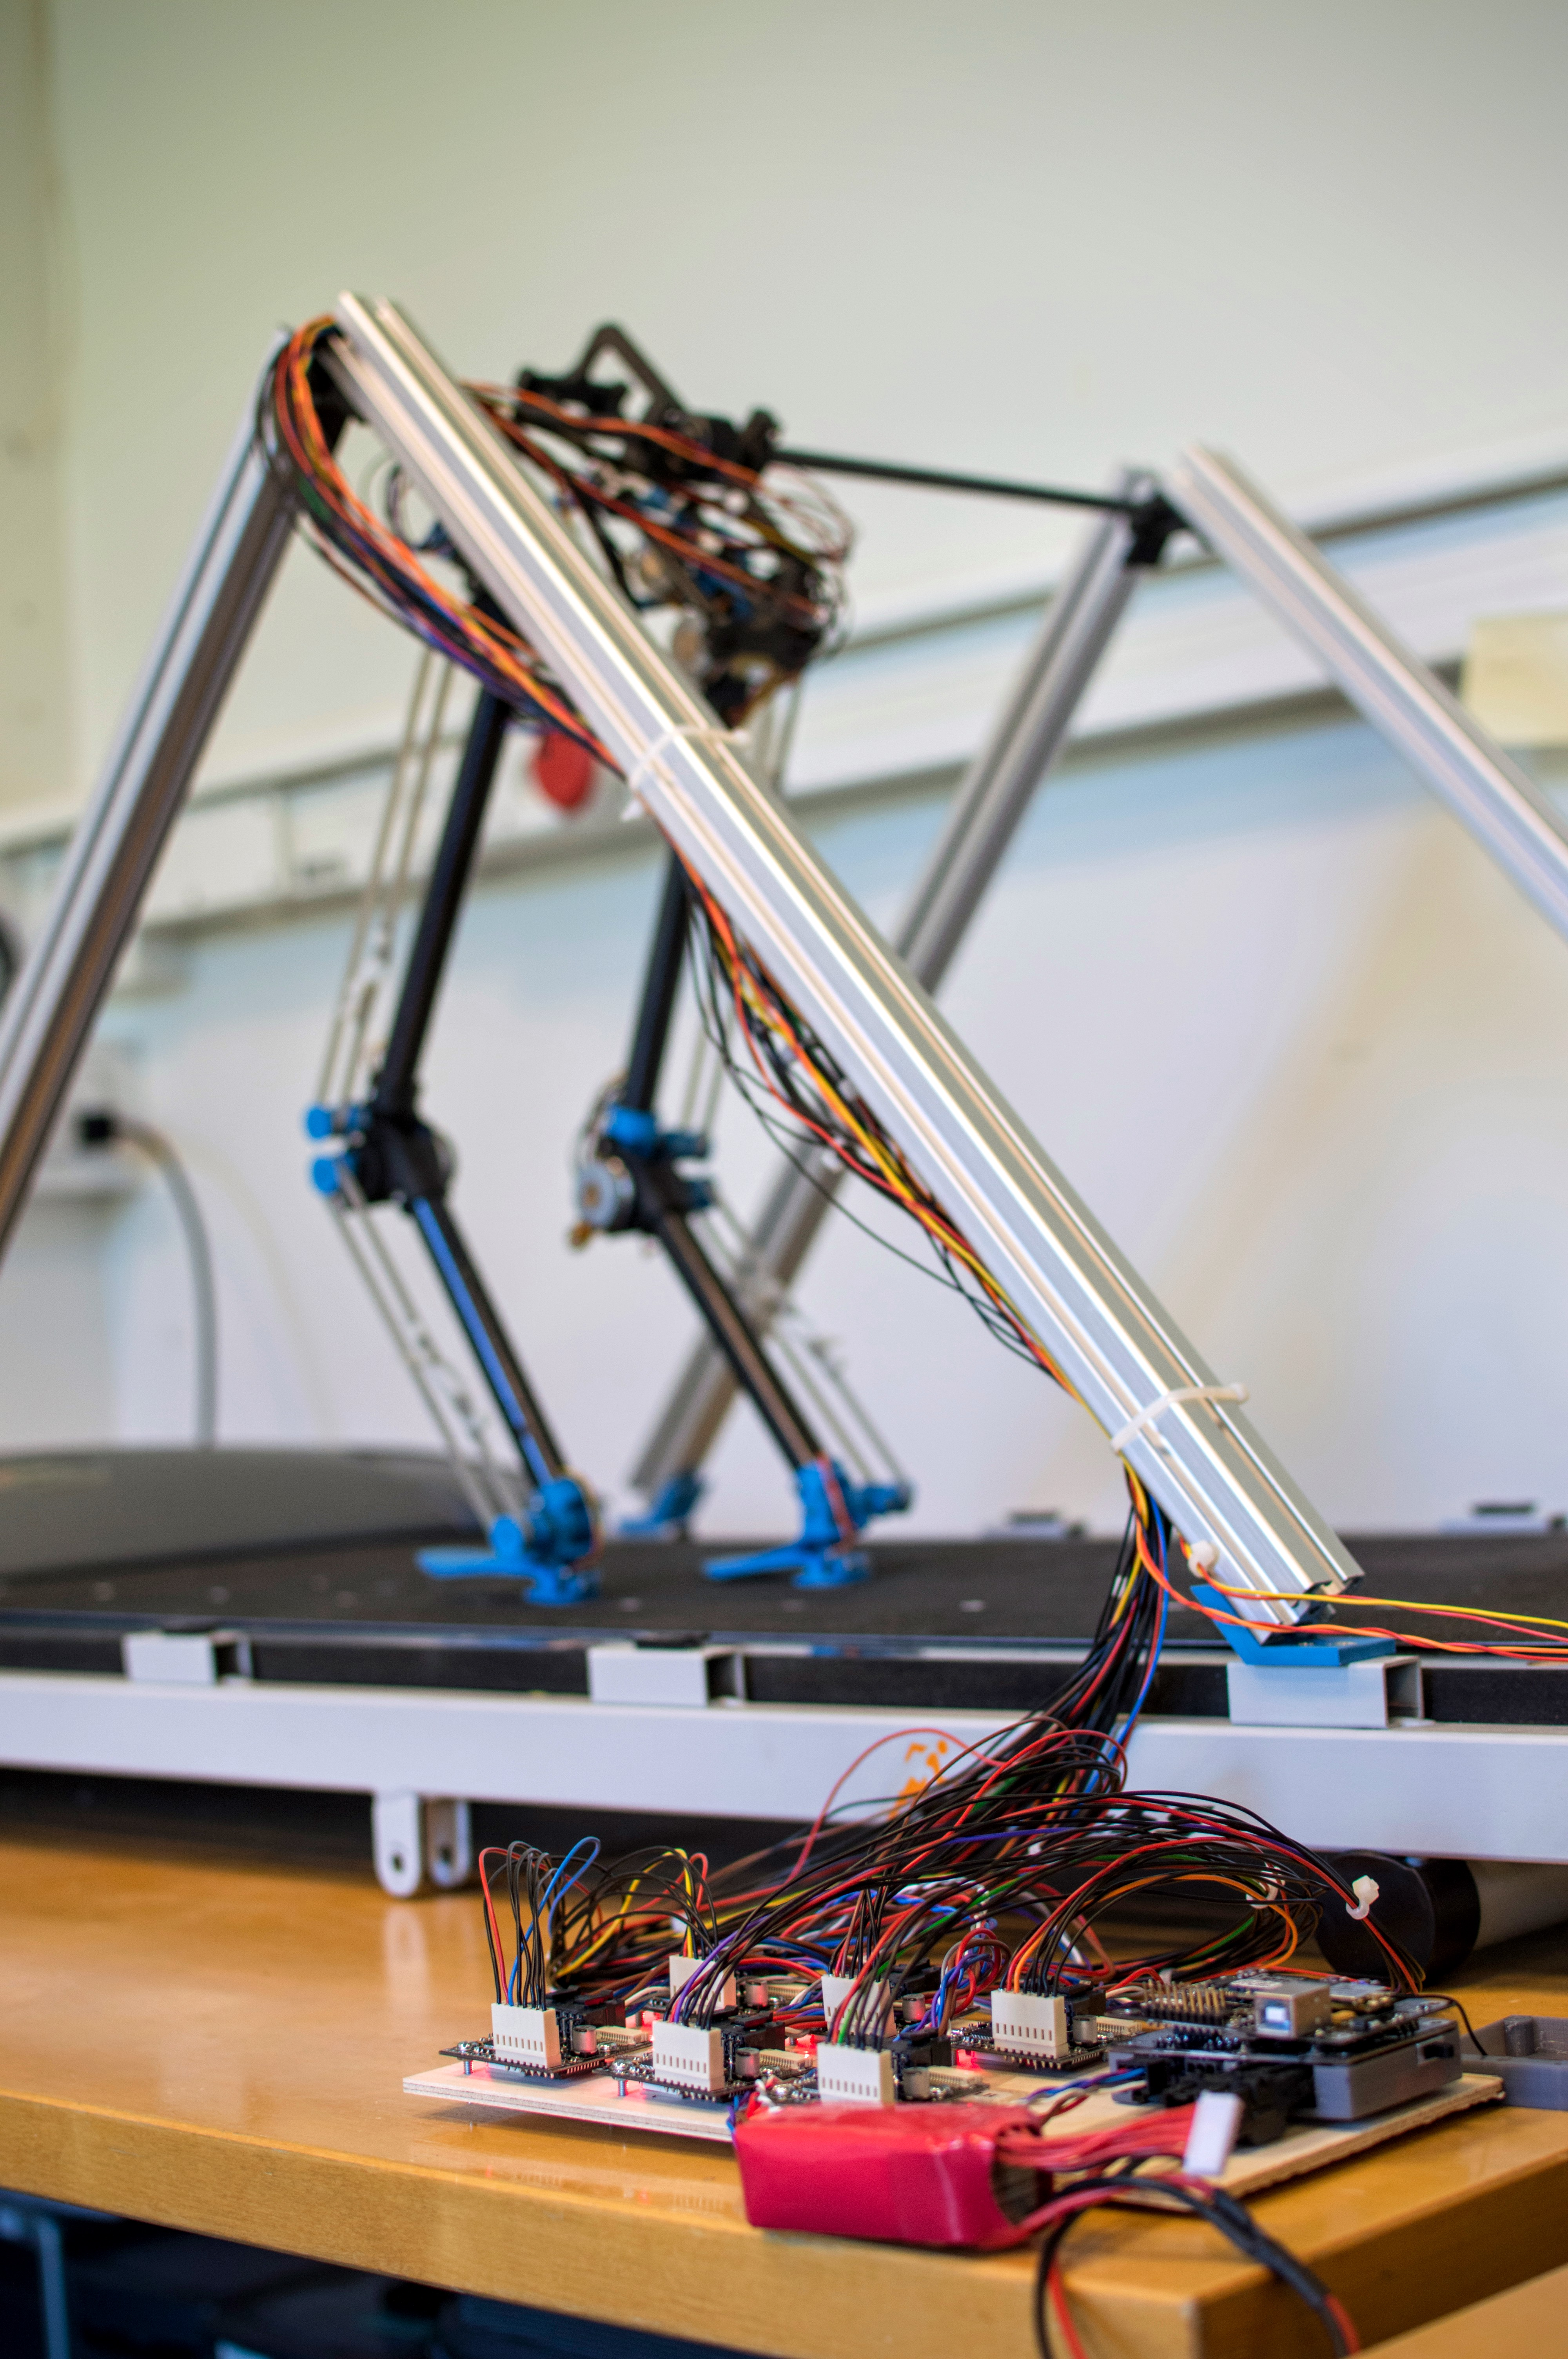
\includegraphics[width=\textwidth]{figures/photo_electronics_2.jpg}
    \caption{Wiring on the structure}
    \label{fig:electronics1}
  \end{subfigure}
  \begin{subfigure}[b]{0.4\textwidth}
    \includegraphics[width=\textwidth]{figures/photo_electronics.jpg}
    \caption{Electronics main board}
    \label{fig:electronics2}
  \end{subfigure}
  \begin{subfigure}[b]{0.4\textwidth}
    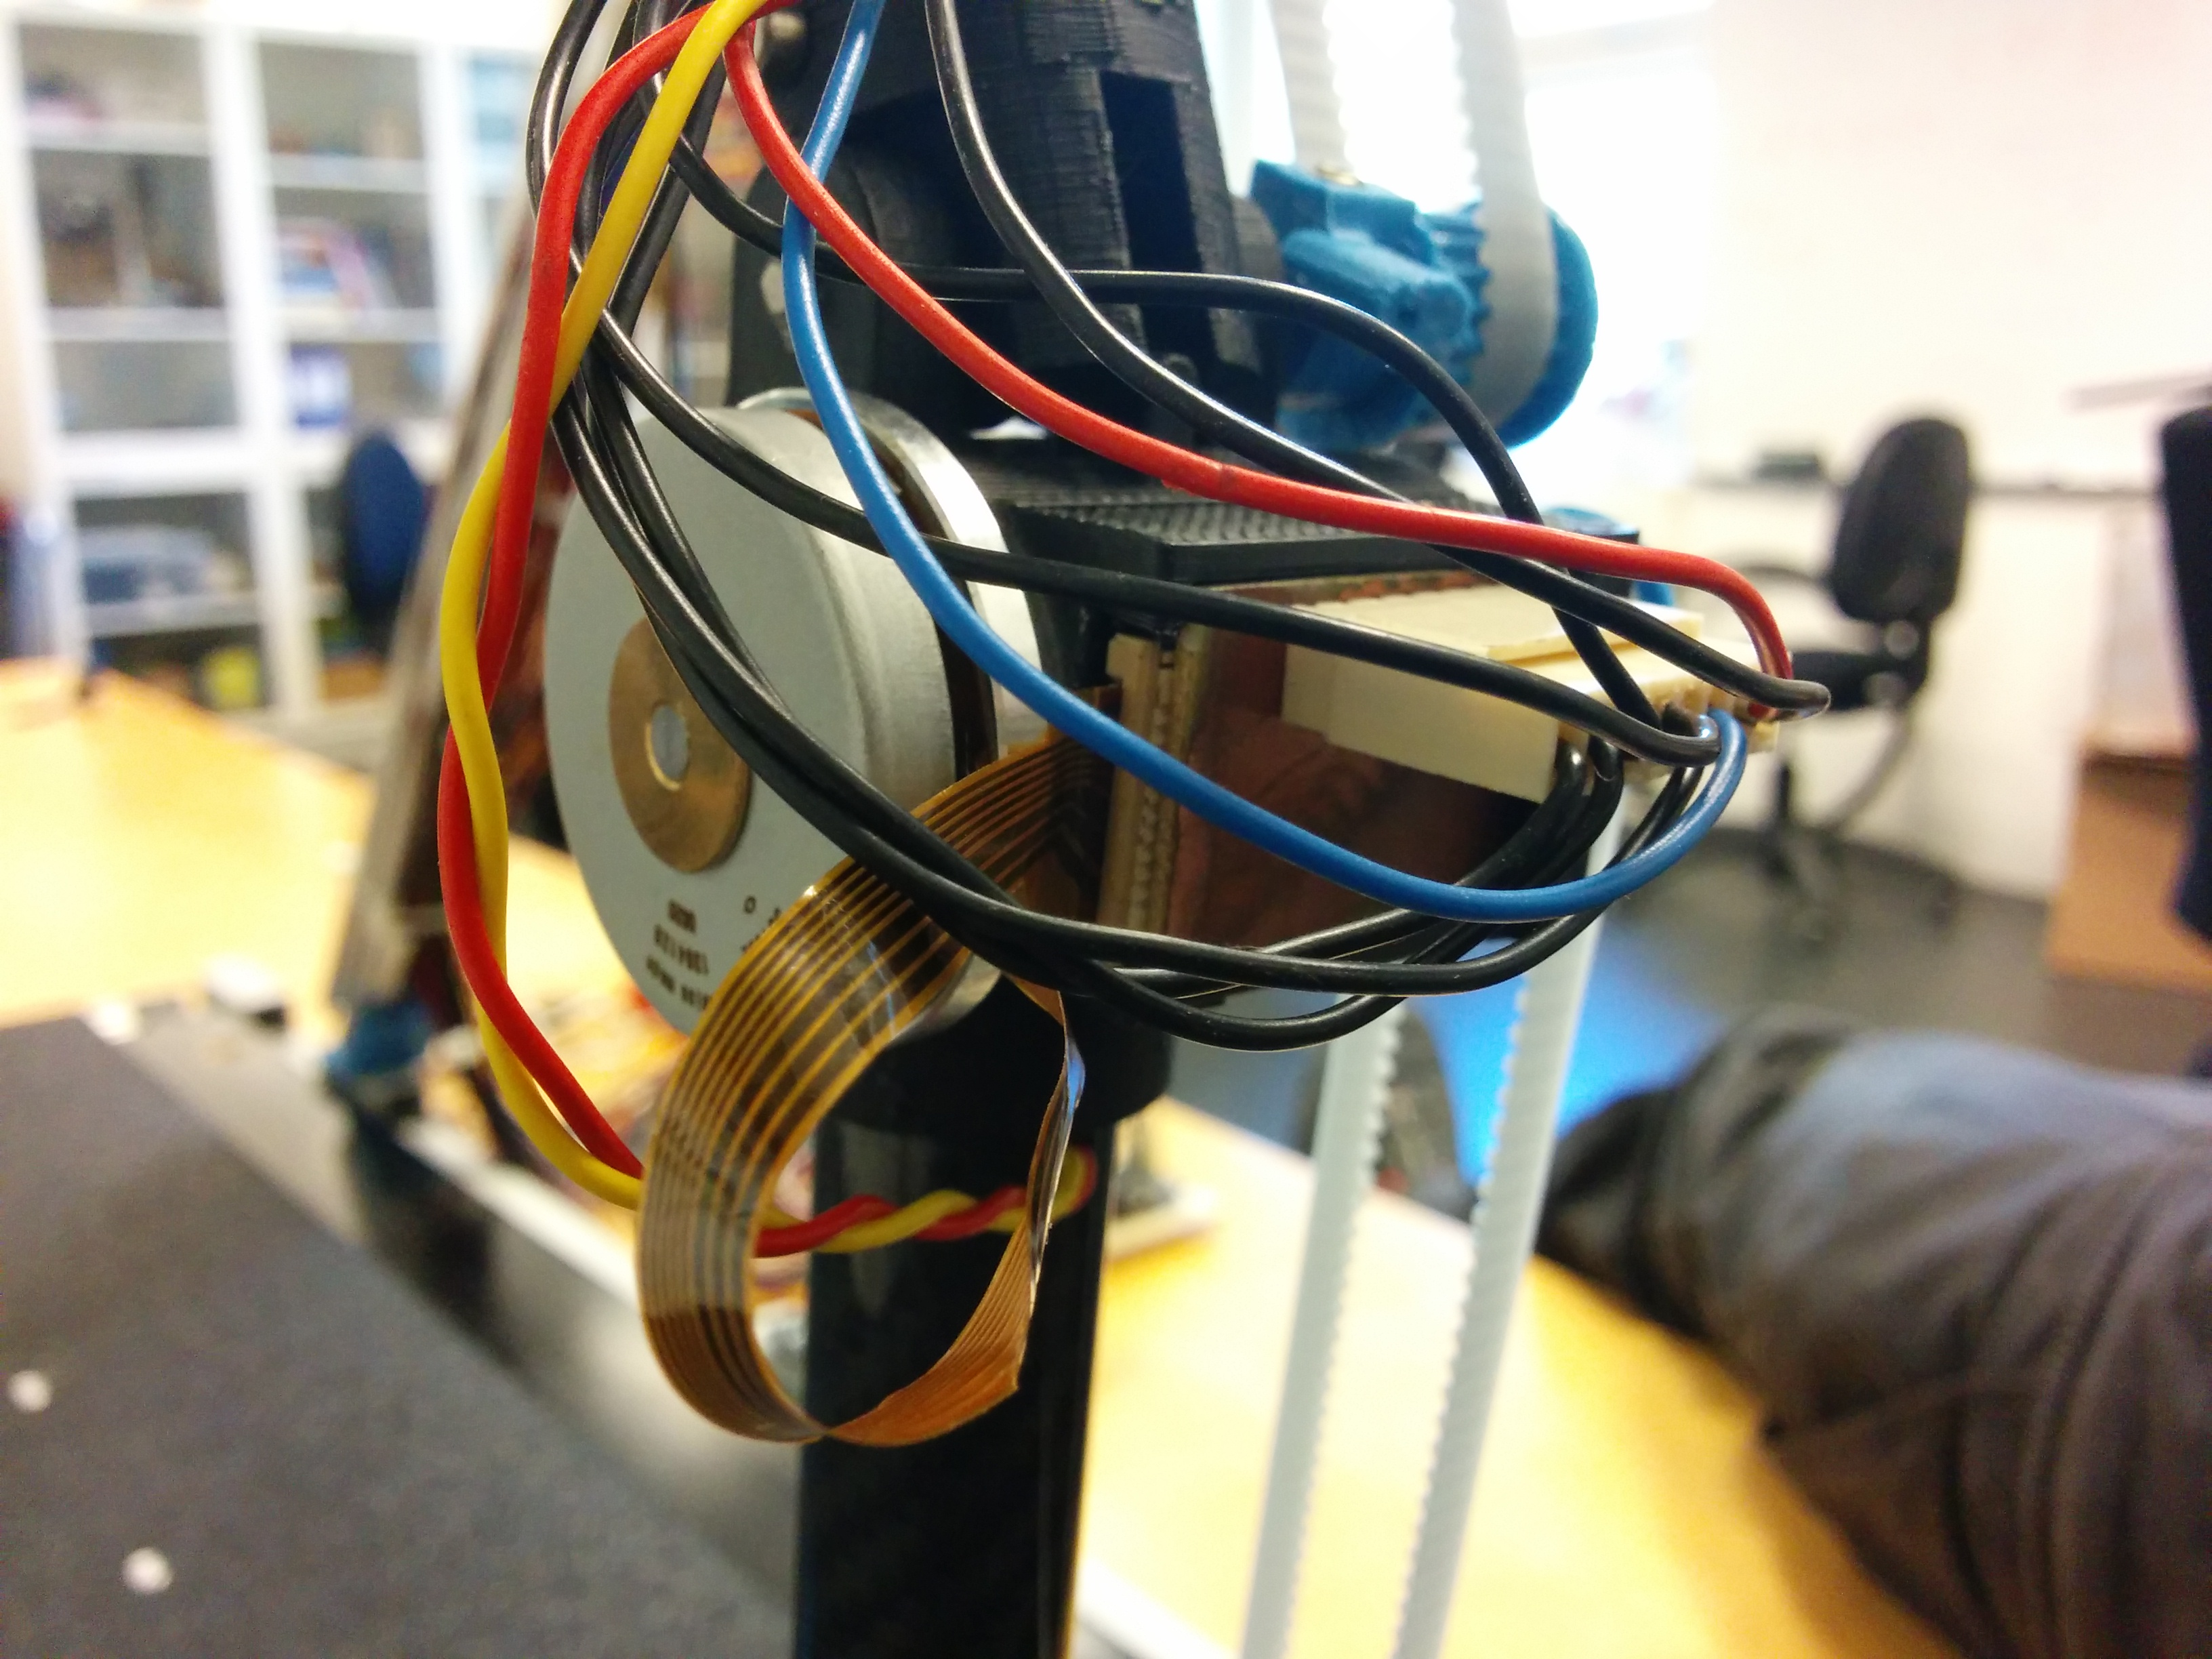
\includegraphics[width=\textwidth]{figures/photo_electronics_detail.jpg}
    \caption{Left leg extension PCB implemented}
    \label{fig:pcb2}
  \end{subfigure}
  \caption{Final architecture of electronics}
\end{figure}

% section pcbs_and_wiring (end)